\section{Experiments}\label{sec:experiments}

\subsection{Relational games}

The \textit{relational games} dataset was contributed as a benchmark for relational reasoning by~\citep{shanahanExplicitlyRelationalNeural}. It consists of a family of binary classification tasks for identifying abstract relational rules between a set of objects represented as images. The objects consist of three sets of simple geometric shapes, referred to as ``pentominoes'', ``hexominoes'', and ``stripes'' (\Cref{fig:relational_games_objects}). The objects are arranged in a $3 \times 3$ grid. Each relational game task corresponds to some relationship between the objects (see~\Cref{tab:relational_games_tasks} and~\Cref{fig:relational_games_tasks}), and the target is to classify whether the relationship holds among a given sequence of objects or not.

In our experiments, we evaluate out-of-distribution generalization by training all models on the pentominoes objects and evaluating on the hexominoes and stripes objects. The input to all models is presented as a sequence of $9$ objects, each represented as a $12 \times 12 \times 3$ RGB image. In all models, the objects are processed independently by a CNN with a shared architecture. This produces a sequence of $9$ $d$-dimensional vectors. The sequence of objects is then passed to the relation-processing component of the model. The results are then flattened and passed through an MLP with a shared architecture to produce the final prediction. We compare four models: a relational convolution model (abbreviated RelConvNet), CoRelNet~\citep{kergNeuralArchitecture2022}, PrediNet~\citep{shanahanExplicitlyRelationalNeural}, and a Transformer~\citep{vaswani2017attention}. The architectural details of each model are described in~\Cref{tab:architectures}.

The pentominoes split of the relational games dataset is used for training. We hold out 1000 samples for validation (during training) and 5000 samples for testing (after training), and use the rest as the training set. The hexominoes and stripes splits are used to test out-of-distribution generalization after training. For each task and model, we train the model for 50 epochs, while tracking training and validation loss and accuracy. We use the categorical cross-entropy loss and the Adam optimizer with learning rate $0.001$, $\beta_1 = 0.9, \beta_2 = 0.999, \epsilon = 10^{-7}$. We use a batch size of 512. For each model and task, we run 5 trials with different random seeds.

\begin{table}[ht]
    \centering
    \begin{tabular}{p{0.2\textwidth}p{0.7\textwidth}}
    \toprule
    Task              & Description                                                                                                                                                                                             \\ \midrule
    \texttt{same}              & Two random cells out of nine are occupied by an object. They are the ``same'' if they have the same color, shape, and orientation (i.e., identical image)                                               \\\hline
    \texttt{occurs}            & The top row contains one object and the bottom row contains three objects. The ``occurs'' relationship holds if at least one of the objects in the bottom row is the same as the object in the top row. \\\hline
    \texttt{xoccurs}           & Same as occurs, but the relationship holds if exactly one of the objects in the bottom row is the same as the object in the top row.                                                                    \\\hline
    \texttt{between}           & The grid is occupied by three objects in a line (horizontal or vertical). The ``between'' relationship holds if the outer objects are the same.                                                         \\\hline
    \texttt{row match pattern} & The first and third rows of the grid are occupied by three objects each. The ``match pattern'' relationship holds if the relation pattern in each row is the same (e.g., AAA, AAB, ABC, etc.)           \\ \bottomrule
\end{tabular}
    \caption{Relational games tasks.}
    \label{tab:relational_games_tasks}
\end{table}

\begin{figure}
    \centering
    \begin{subfigure}[t]{0.37\textwidth}
        \centering
        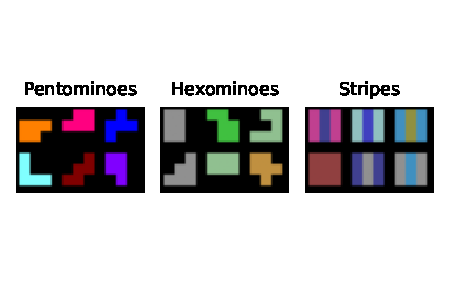
\includegraphics[width=\textwidth]{figs/relational_games_objects.pdf}
        % \caption{Examples of objects from each split.}
        \label{fig:relational_games_objects}
    \end{subfigure}
    \begin{subfigure}[t]{0.62\textwidth}
        \centering
        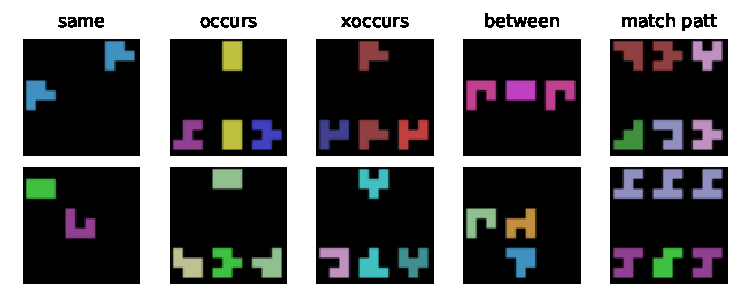
\includegraphics[width=\textwidth]{figs/relational_games_tasks.pdf}
        % \caption{Examples of problem instances for each task. The top row is an example where the relation holds and the bottom row is an example where the relation does not hold.}
        \label{fig:relational_games_tasks}
    \end{subfigure}
    \caption{Relational games dataset.~\textbf{Left} Examples of objects from each split.~\textbf{Right} Examples of problem instances for each task. The top row is an example where the relation holds and the bottom row is an example where the relation does not hold.}
    \label{fig:relational_games_dataset}
\end{figure}

\begin{table}[ht]
    \centering
    \begin{tabular}{p{0.2\textwidth}p{0.8\textwidth}}
    \toprule
    Model / Component & Architecture                                                                                                                                                                                                                                                                                       \\ \midrule
    Common CNN        & \texttt{Conv2D} $\to$ \texttt{MaxPool2D} $\to$ \texttt{Conv2D} $\to$ \texttt{MaxPool2D} $\to$ \texttt{Flatten}. \\
    & \texttt{Conv2D}: num filters = 16, filter size = $3 \times 3$, activation = relu. \\
    & \texttt{MaxPool2D}: stride = 2. \\\hline
    RelConvNet        & \texttt{CNN} $\to$ \texttt{MHR} $\to$ \texttt{RelConv} $\to$ \texttt{Flatten} $\to$ \texttt{MLP}. \\
    & \texttt{MHR}: relation dim = 16, projection dim = 4, symmetric. \\
    & \texttt{RelConv}: num filters = 16, filter size = 3, discrete groups = combinations. \\\hline
    CoRelNet          & \texttt{CNN} $\to$ \texttt{CoRelNet} $\to$ \texttt{Flatten} $\to$ \texttt{MLP}. \\
    & Standard CoRelNet has no hyperparameters. \\\hline
    PrediNet          & \texttt{CNN} $\to$ \texttt{PrediNet} $\to$ \texttt{Flatten} $\to$ \texttt{MLP}. \\
    & \texttt{PrediNet}: key dim = 4, number of heads = 4, num relations = 16. \\\hline
    Transformer       & \texttt{CNN} $\to$ \texttt{TransformerEncoder} $\to$ \texttt{AveragePooling} $\to$ \texttt{MLP}. \\
    & \texttt{TransformerEncoder}: num layers = 1, num heads = 8, feedforward intermediate size = 32, activation = relu. \\\hline
    Common output MLP & \texttt{Dense(64, activation='relu')} $\to$ \texttt{Dense(2)}.                                                                                                                                                                                                              \\ \bottomrule
\end{tabular}
    \caption{Model architectures.}
    \label{tab:architectures}
\end{table}



\begin{figure}
    \centering
    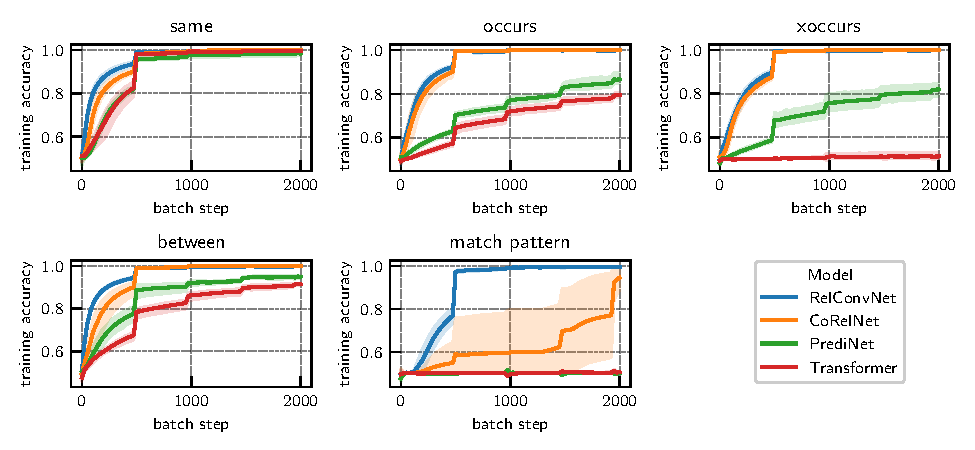
\includegraphics[width=\textwidth]{figs/experiments/all_training_curves.pdf}
    \caption{Training curves for each relational games task. Showing curves up to 2,000 batch steps. Solid lines indicate the mean over 5 trials and the shaded regions indicate a bootstrap 95\% confidence interval.}\label{fig:training_curves}
\end{figure}

\textbf{Sample efficiency.} We observe that the relational inductive biases of RelConvNet, and relational models more generally, grant a significant advantage in sample-efficiency.~\Cref{fig:training_curves} shows the training accuracy over the first 2,000 batches for each model. RelConvNet, CoRelNet, and PrediNet are explicitly relational architectures, whereas the Transformer is not. The Transformer is able to process relational information through its attention mechanism, but this information is entangled with the features of individual objects (which, for these relational tasks, is extraneous information). The Transformer consistently requires the largest amount of data to learn the relational games tasks. PrediNet tends to be more sample-efficient. RelConvNet and CoRelNet are the most sample-efficient, with RelConvNet only slightly more sample-efficient on the `same', `occurs', `xoccurs', and `between' tasks.

On the `match pattern' task, however, RelConvNet is significantly more sample-efficient. We attribute this to the fact that RelConvNet is able to model higher-order relations through its relational convolution module. The `match pattern' task can be thought of as a simple second-order relational tasks---it involves computing relations between two groups objects, and comparing those relations between the two groups. The relational convolution module naturally models this kind of situation since it considers groups of objects and describes the relations between them. The performance we observe here indicates that the relational games dataset is in some sense saturated by models like RelConvNet and CoRelnet and that more complex relational benchmarks are needed to evaluate this class of models. In particular, benchmarks which test the ability to model higher-order relations.

\begin{table}
    \centering
    \begin{tabular}{llll}
\toprule
              &             &     Hexos Accuracy &   Stripes Accuracy \\
Task & Model &                    &                    \\
\midrule
same & RelConvNet &  $0.989 \pm 0.002$ &  $0.974 \pm 0.003$ \\
              & CoRelNet &  $0.988 \pm 0.006$ &  $0.724 \pm 0.112$ \\
              & PrediNet &  $0.990 \pm 0.004$ &  $0.983 \pm 0.007$ \\
              & Transformer &  $0.997 \pm 0.001$ &  $0.993 \pm 0.004$ \\\hline
occurs & RelConvNet &  $0.980 \pm 0.001$ &  $0.880 \pm 0.015$ \\
              & CoRelNet &  $0.992 \pm 0.004$ &  $0.518 \pm 0.012$ \\
              & PrediNet &  $0.907 \pm 0.020$ &  $0.775 \pm 0.046$ \\
              & Transformer &  $0.881 \pm 0.015$ &  $0.724 \pm 0.021$ \\\hline
xoccurs & RelConvNet &  $0.967 \pm 0.001$ &  $0.946 \pm 0.006$ \\
              & CoRelNet &  $0.980 \pm 0.007$ &  $0.606 \pm 0.035$ \\
              & PrediNet &  $0.872 \pm 0.036$ &  $0.810 \pm 0.028$ \\
              & Transformer &  $0.867 \pm 0.017$ &  $0.753 \pm 0.031$ \\\hline
between & RelConvNet &  $0.991 \pm 0.001$ &  $0.988 \pm 0.002$ \\
              & CoRelNet &  $0.995 \pm 0.001$ &  $0.582 \pm 0.063$ \\
              & PrediNet &  $0.978 \pm 0.006$ &  $0.950 \pm 0.019$ \\
              & Transformer &  $0.986 \pm 0.003$ &  $0.961 \pm 0.010$ \\\hline
match pattern & RelConvNet &  $0.961 \pm 0.015$ &  $0.870 \pm 0.041$ \\
              & CoRelNet &  $0.942 \pm 0.011$ &  $0.581 \pm 0.026$ \\
              & PrediNet &  $0.710 \pm 0.040$ &  $0.658 \pm 0.053$ \\
              & Transformer &  $0.627 \pm 0.005$ &  $0.591 \pm 0.006$ \\
\bottomrule
\end{tabular}

    \caption{Out-of-distribution Generalization results on relational games. We report means $\pm$ standard error of mean over 5 trials.}\label{tab:ood_generalization}

\end{table}

\begin{figure}
    \begin{subfigure}{0.5\textwidth}
        \centering
        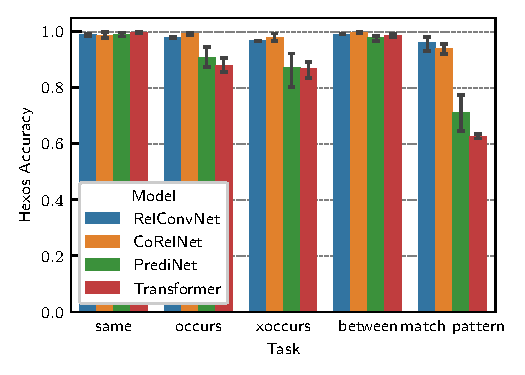
\includegraphics[width=\textwidth]{figs/experiments/hexos_acc.pdf}
        \caption{OoD generalization on Hexos objects}\label{fig:ood_generalization_hexos}
    \end{subfigure}
    \begin{subfigure}{0.5\textwidth}
        \centering
        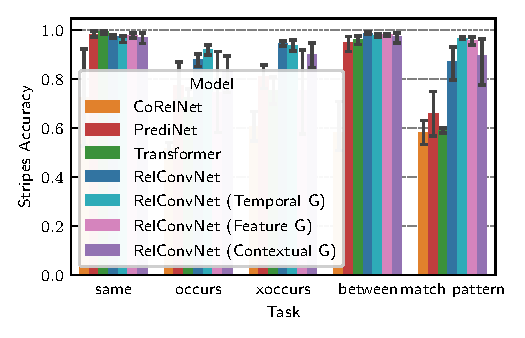
\includegraphics[width=\textwidth]{figs/experiments/stripes_acc.pdf}
        \caption{OoD generalization on Stripes objects}\label{fig:ood_generalization_stripes}
    \end{subfigure}
    \caption{Out-of-distribution generalization on hold-out object sets. Bar heights indicate the mean over 5 trials and the errror bars indicate a bootstrap 95\% confidence interval.}\label{fig:ood_generalization}
\end{figure}

\textbf{Out-of-distribution generalization}~\Cref{fig:ood_generalization} and~\Cref{tab:ood_generalization} report model performance on the two hold-out object sets after training. On the hexominoes objects, which are similar-looking to the pentominoes objects used for training, RelConvNet and CoRelNet do nearly perfectly. PrediNet and the Transformer do well on the simpler tasks, but struggle with the more difficult `match pattern' task. The stripes objects are visually more distinct from the pentominoes of the training split, making generalization more difficult. We observe an overall drop in performance for all models. The drop is particularly dramatic for CoRelNet\footnote{Unlike~\citep{kergNeuralArchitecture2022}, we do not use temporal context normalization in our experiments. We believe this is the more appropriate choice for evaluating relational architectures such as RelConvNet and CoRelNet since TCN is an added confounder. We discuss this more in~\Cref{sec:tcn_discussion}.}. We conjecture that this is due to CoRelNet's inability to model multi-dimensional relations, necessitating that all relational information is squeezed into a scalar quantity. \texttt{TODO: elaborate or remove this comment?}. The separation between RelConvNet and the other models is largest on the ``match pattern'' task of the stripes split (the most difficult task and the most difficult generalization split). Here, RelConvNet maintain a mean accuracy of 87\% while the other models drop below 65\%. We conjecture that this is due to RelConvNet's natural ability to model such higher-order relations as well as its ability to model multi-dimensional relations.


\subsection{`SET': grouping and compositionality in relational reasoning}\label{ssec:experiments_set}

`SET' is a card game which forms a simple but challenging relational task. The `objects' are a set cards each representing four attributes which can take one of three values each. `Color' can be red, green, or purple; `number' can be one, two, or three; `shape' can be diamond, squiggle, or oval; and `shading' can be solid, striped, or empty. A `set' is a triplet of cards such that for each attribute, the attribute is either the same on all three cards or different on all three cards.~\Cref{fig:set_example} shows a sample of SET cards.

\begin{wrapfigure}{R}{0.25\textwidth}
	\vskip-5pt
	\begin{tabular}{c}
		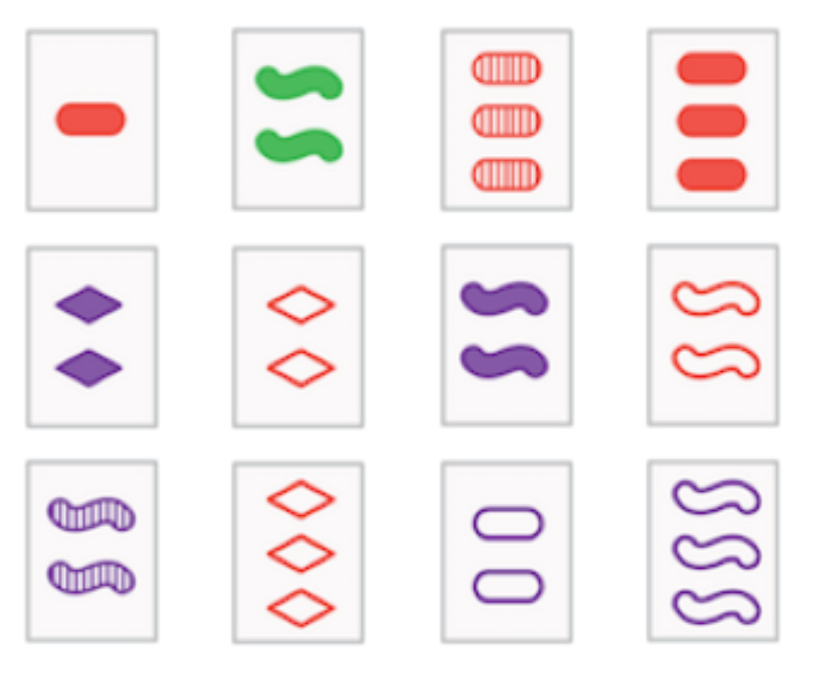
\includegraphics[width=.25\textwidth]{figs/set_example}\\[-5pt]
	\end{tabular}
	\caption{\footnotesize The SET game}\label{fig:set_example}
\end{wrapfigure}
In SET, the task is: given a hand of $k > 3$ cards, find a `set' among them (typically, SET is played with $k=12$, with two players competing to find a `set' first). This task is deceptively challenging, and is representative of the type of relational reasoning that humans excel at but machine learning systems still struggle with. To solve the task, one must process the sensory information of individual cards to identify the values of each attribute, then somehow search over combinations of cards and reason about the relations between them. Importantly, this type of relational reasoning requires attending over several attributes and relations simultaneously while representing some notion of `groups'.  The construct of relational convolutions proposed in this paper is a step towards developing machine learning systems which can perform this kind of relational reasoning.


In this section, we evaluate RelConvNet on a task based on `SET' and compare it to several baselines. The task is: given a sequence of $k=5$ images of SET cards, determine whether or not they contain a `set'. All models share the common architecture $(x_1, \ldots, x_k) \to \texttt{CNN} \to \{ \cdot \} \to \texttt{MLP} \to \hat{y}$, where $\{\cdot\}$ is RelConvNet, CoRelNet, PrediNet, or a Transformer. The architectures are identical to the previous section (described in~\Cref{tab:architectures}) with the exception that RelConvNet uses the permutation-invariant version of the relational inner product (\Cref{eq:symmetric_relational_inner_prod}) with max-pooling, and the projection dimension is changed to $16$ to better match the larger embedding dimension of the card images. The CNN embedder is pre-trained on the task of classifying the four attributes of the cards and an intermediate layer is used to generate embeddings of dimension $64$ for each card. The parameters of the CNN are fixed is used for all models. Similarly, the output MLP architecture is shared across all models. It consists of two hidden layers with $64$ and $32$ neurons, respectively, and ReLU activations.

\begin{wrapfigure}{R}{0.4\textwidth}
    \centering
    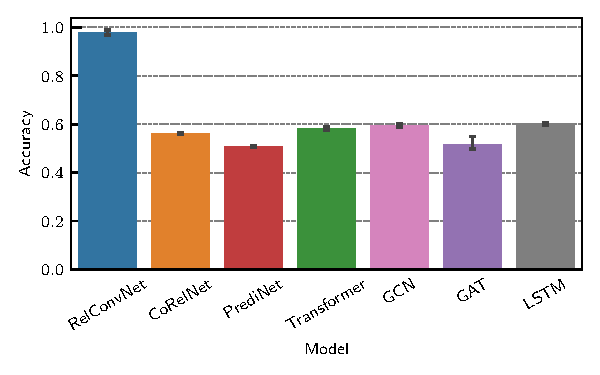
\includegraphics[width=0.4\textwidth]{figs/experiments/contains_set_acc.pdf}
    \caption{\footnotesize Hold-out test accuracy. Error bars indicate 95\% bootstrap confidence intervals.}\label{fig:contains_set_acc}
\end{wrapfigure}

In SET, there exists $\binom{81}{3} = 85\,320$ triplets of cards, of which $1\,080$ are a `set' ($1/79{}^{\mathrm{th}}$). We partition the `sets' into training (70\%), validation (15\%), and test (15\%) sets. The training, validation, and test datasets are generated by sampling $k$-tuples of cards such that with probability $1/2$ the $k$-tuple does not contain a set, and with probability $1/2$ it contains a set among the corresponding partition of sets. Partitioning the data in this way allows us to measure the models' ability to ``learn the rule'' and identify new unseen `sets'. We train for 100 epochs with the same loss, optimizer, and batch size as the experiments in the previous section.~\Cref{fig:contains_set_acc} shows the hold-out test accuracy for each model.~\Cref{fig:contains_set_training_curves} shows the training and validation accuracy over the course of training.

\begin{figure}
    \begin{subfigure}{0.5\textwidth}
        \centering
        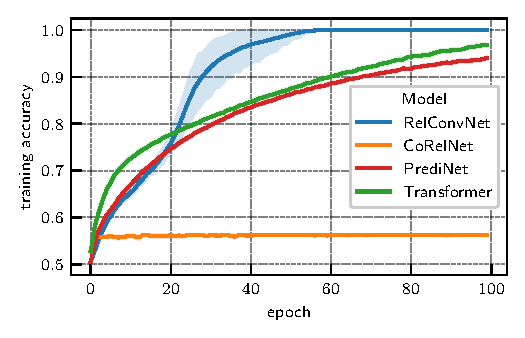
\includegraphics[width=\textwidth]{figs/experiments/contains_set_training_curves_trainacc.pdf}
        \caption{Training accuracy over the course of training.}\label{fig:contains_set_training_curves_trainacc}
    \end{subfigure}
    \begin{subfigure}{0.5\textwidth}
        \centering
        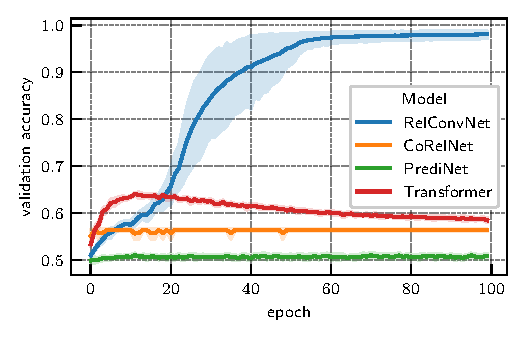
\includegraphics[width=\textwidth]{figs/experiments/contains_set_training_curves_valacc.pdf}
        \caption{Validation accuracy over the course of training.}\label{fig:contains_set_training_curves_valacc}
    \end{subfigure}
    \caption{Training curves for the ``contains SET'' experiments. Solid lines indicate the mean over 10 trials. Shaded regions represent a 95\% bootstrap confidence interval.}\label{fig:contains_set_training_curves}
\end{figure}

We observe that RelConvNet is able to learn the task and generalize to new `sets' with near-perfect accuracy. On the other hand, CoRelNet and the Transformer have accuracies only slightly better than random guessing on the test set, while PrediNet learns nothing that generalizes to the test set. The picture becomes more clear when looking at training curves. While the Transformer and PrediNet are eventually able to fit the training data, it is unable to ``learn the rule'' in a way the generalizes to the validation or test set. This suggests that the Transformer architecture has the function-approximation capabilities to fit a wide array of sequence-tasks, but it does not have the right inductive biases for relational reasoning. A possible explanation is that relations are processed only implicitly through its attention mechanism, rather than explicitly via a relation tensor. Moreover, it does not naturally support reasoning about the relations between groups of objects. These are strengths of the relational convolutional networks architecture.